\section{Futures und Promises}

\subsection{Motivation}

\paragraph{Blockierende Methodenaufrufe} Methodenaufrufe in üblichen Programmiersprachen sind blockierend. Das bedeutet,
dass das Hauptprogramm solange blockiert wird wie der Methodenaufruf läuft.
So wird in Listing \ref{lst:codeBlocking} die Methode \texttt{tuEtwas()} eines Objektes aufgerufen.

\begin{lstlisting}[caption={Blockierender Methodenaufruf},label={lst:codeBlocking},captionpos=b]
main() {
  objekt.tuEtwas()
  tuEtwasAnderes()
}
\end{lstlisting}

\begin{figure}[htbp]
  \centering
	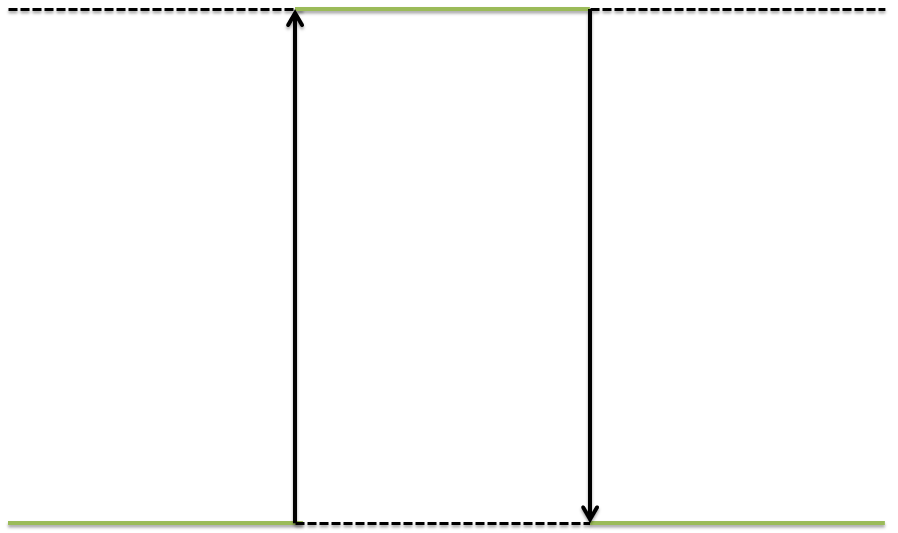
\includegraphics[scale=0.6]{pic/BlockingCall.png}
  \caption{Ein blockierender Methodenaufruf }
  \label{blockingCall}
\end{figure}

In Abbildung \ref{blockingCall} wird dieser Sachverhalt graphisch
veranschaulicht: Da der Aufrufer blockiert wird solange der Aufgerufene
arbeitet, kann immer nur ein Thread arbeiten.

Besonders in der heutigen Zeit, in der immer mehr Computer mehrere
Prozessorkerne haben, ist dieses Verhalten nicht erwünscht. Doch auch
auf einem Computer mit nur einem Prozessor kann es erforderlich sein,
nebenläufig zu programmieren.

\paragraph{Nicht-blockierende Methodenaufrufe} Führen wir das Schlüsselwort
\texttt{nebenlaeufig} in unseren Pseudocode ein,
können wir ausdrücken, dass die aufgerufene Methode nicht blockieren soll
und im Hauptthread weitergearbeitet werden kann.

\begin{lstlisting}[caption={Nebenläufiger Methodenaufruf},label={lst:codeConcurrent},captionpos=b]
main() {
  nebenlaeufig objekt.tuEtwas()
  tuEtwasAnderes()
}
\end{lstlisting}

\begin{figure}[htbp]
  \centering
	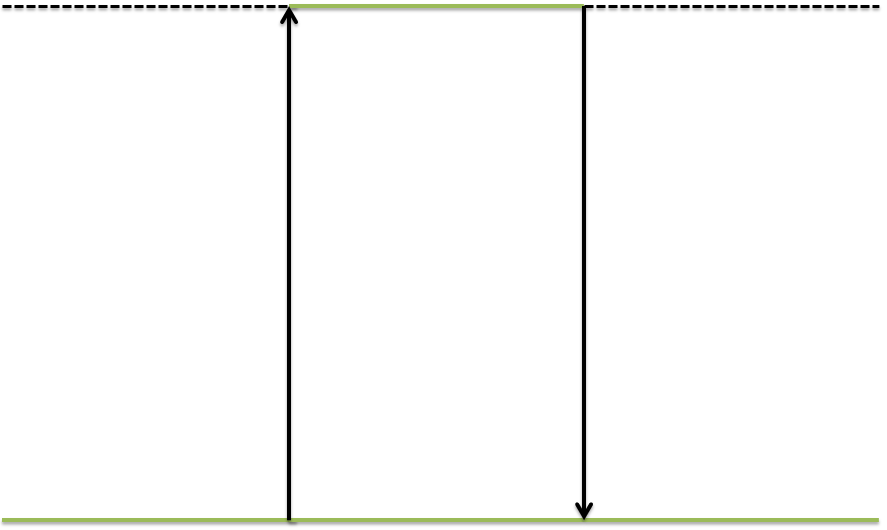
\includegraphics[scale=0.6]{pic/NonBlockingCall.png}
  \caption{Ein nicht blockierender Methodenaufruf }
  \label{nonBlockingCall}
\end{figure}

Nun kann \texttt{tuEtwasAnderes()} \emph{nebenläufig} ausgeführt werden. Damit
ist es bei mehreren Prozessoren möglich, den Code parallel auszuführen.

Abbildung \ref{nonBlockingCall} zeigt das gewünschte Verhalten:
Es entstehen zwei Threads die gleichzeitig ausgeführt werden können,
wenn die Hardware dazu in der Lage ist.

Eine Analogie aus dem IT-Umfeld sind Unix-Shells. Wenn zum Beispiel ein
\texttt{find}-Befehl ausgeführt wird, blockiert die Shell bis der Befehl
abgeschlossen ist. Durch Anhängen eines kaufmännischen \glqq und\grqq{}-Zeichens 
ist es möglich,
den Befehl im Hintergrund laufen zu lassen. Dadurch kann im selben
Terminal weiter gearbeitet werden während der Befehl im Hintergrund
läuft.

Klar ist, dass diese Technik keine Wunder bewirken kann und die zur
Verfügung stehenden Ressourcen nicht vervielfacht, dennoch können
sie so besser ausgenutzt werden da der Prozessor weniger häufig
in einen Zustand kommt in dem er keine Arbeit hat.

\subsection{Futures}

Im SIP-14 wird ein \emph{Future} wie folgt beschrieben:
\begin{quote}
Futures provide a nice way to reason about performing many operations in 
parallel – in an efficient and non-blocking way. The idea is simple, a Future 
is a sort of placeholder object that you can create for a result that doesn’t 
yet exist. Generally, the result of the Future is computed concurrently and can 
be later collected. Composing concurrent tasks in this way tends to result in 
faster, asynchronous, non-blocking parallel code.

A Future object either holds a result of a computation or an 
exception in the case that the computation failed.
\end{quote}

Ein \emph{Future} ist eine Abstraktion für einen \emph{Thread}.
Dabei werden viele technische Details vor dem Anwendungsentwickler
versteckt, um die man sich zum Beispiel bei der Arbeit mit klassischen
Threads in Programmiersprachen wie \emph{Java} kümmern muss.

Wichtig hervorzuheben sind die Begriffe \emph{non-blocking} und
\emph{placeholder object}.

Auf die Eigenschaften von nicht blockierenden Aufrufen wurde bereits
im vorhergehenden Abschnitt eingegangen. \emph{Futures} sind so konzipiert,
dass sie nicht blockierend arbeiten, aber wenn es erforderlich ist
kann trotzdem blockiert werden bis ein \emph{Future} fertig ist.

Der Begriff \emph{placeholder object} sagt aus, wie das mentale
Modell hinter dem Konzept \emph{Future} zu verstehen ist. Ein
\emph{Future} ist ein Behältnis, welches irgendwann einen Wert
beinhalten wird. Es ist nicht möglich zu sagen wie lange das dauern
wird, es ist aber möglich zu erfahren ob dieser Wert bereits
verfügbar ist. Wenn er verfügbar ist, dann kann er beliebig oft
gelesen, aber nie überschrieben werden.

Wichtig zu erwähnen ist, dass ein \emph{Future} alternativ
auch eine Exception beinhalten kann. Dies ist zum Beispiel sinnvoll
wenn bei der Berechnung etwas schief geht oder um zu signalisieren
dass ein definierter Fehlerzustand erreicht wurde.

Alles was innerhalb eines \emph{Futures} passiert läuft nicht im
Hauptthread.

\paragraph{Einfaches Beispiel in Pseudocode}

\lstinputlisting
    [caption={Pseudocode zum Minimalbeispiel eines Futures },
       label = lst:scala_mini_future,
       captionpos=b]
 {../code/minimal/future/Future.pseudo}
 
In Listing \ref{lst:scala_mini_future} ist der Umgang mit einem \emph{Future}
skizziert. Sie sind generische Typen, es ist also möglich \emph{Futures}
zu verwenden, die beliebige Typen beinhalten. Der Code des \emph{Futures}
wird innerhalb des \texttt{future \{ ... \}}-Blocks definiert. Der
Rückgabewert muss dem Typen entsprechen, den der \emph{Future} zurückgibt.

Die Verarbeitung des Ergebnisses kann in der \texttt{onComplete}-Callback-Methode 
erfolgen. Um nur auf erfolgreiche oder erfolglose Komplettierungen
zu reagieren, gibt es die \texttt{onSuccess}- bzw. \texttt{onFailure}-Methoden,
welche das Abprüfen auf Erfolg ersparen.

\subsection{Promises}

Ein \emph{Promise} hingegen wird im SIP-14 folgendermaßen beschrieben:
\begin{quote}
A promise can be thought of as a writeable, single-assignment container, which 
completes a future. That is, a promise can be used to successfully complete a 
future with a value (by \glqq completing\grqq{} the promise) using the \texttt{success} method. 
Conversely, a promise can also be used to complete a future with an exception, 
by failing the promise, using the \texttt{failure} method.
\end{quote}

Das Konzept \emph{Promise} baut auf den \emph{Futures} auf. Es bietet
einmaligen Schreibzugriff auf ein Objekt, das zum gegebenen Zeitpunkt
noch nicht beschrieben werden kann, zum Beispiel weil dieser Wert
noch nicht berechnet worden ist.

Er befindet sich immer in einem von zwei Zuständen:
\begin{itemize}
 \item{\textbf{\emph{Unerledigt}} Es wurden noch keine Ergebnisse in den Promise geschrieben.}
 \item{\textbf{\emph{Erledigt}} Der Promise wurde durch ein Ergebnis oder durch eine Exception abgeschlossen.}
\end{itemize}

\paragraph{Einfaches Beispiel in Pseudocode}

\lstinputlisting
    [caption={Pseudocode zum Minimalbeispiel eines Promises },
       label = lst:scala_mini_promise,
       captionpos=b]
 {../code/minimal/promise/Promise.pseudo}
 
Im Beispiel in Listing \ref{lst:scala_mini_promise} ist ein \emph{Promise} zu sehen.
Jedes \emph{Promise} beinhaltet ein \emph{Future}. Im Programm kann
so lange gerechnet werden bis der Wert, mit dem das \emph{Promise}
vervollständigt werden kann, verfügbar ist. Im Beispiel ist dieser
Wert der Einfachheit halber hart codiert, in der Praxis wird er das
nicht sein.

\paragraph{Vergleich} von \emph{Futures} und \emph{Promises}.

\begin{table}[h]
\begin{tabular}{lllll}
 & \textbf{Eigenschaft} & \textbf{Future} & \textbf{Promise} &  \\
 & Teil der Scala 2.10 Standardimplementierung & Ja & Ja &  \\
 & Lesbar (mehrfach) & Ja & Nein &  \\
 & Schreibbar (einmal) & Nein & Ja &  \\
 & Beinhaltet anderen & Nein & Ja &  \\
 & Kombinierbar & Ja & Nein &  \\
\end{tabular}
\end{table}

\subsection{Kombinatoren}

\paragraph{Motivation} Kombinatoren werden in der offiziellen 
\emph{Scala}-Dokumentation beschrieben (vgl.: \cite{scalaDokuFP}).
Sie erlauben es, mehrere \emph{Futures} zu verbinden. 
Auf diese Weise können komplexe Zusammenhänge relativ einfach
im Code formuliert werden.

Eine angenehme Eigenschaft von Kombinatoren ist es, dass man bei
der Arbeit damit in der Welt der Futures bleibt. So bildet
ein \emph{map} einen Future auf einen anderen ab. Es gibt keinen
Bruch innerhalb der Programmiersprache, das mentale Modell der
Futures bleibt intakt.

Sie ersparen es dem Programmierer zudem, seinen Code mit verschachtelten
Callback-Methoden auszustatten. Diese machen Programme nicht nur
schwer lesbar, sie vermindern zudem die Sichtbarkeit von \emph{Futures}
die innerhalb eines geschachtelten Blocks erzeugt werden, so dass
außerhalb dieser Ebene nicht auf den Callback dieses \emph{Futures}
reagiert werden kann.

Ein Beispiel für \emph{Futures} mit Kombinatoren ist in \ref{lst:holiday}
gegeben. Ein äquivalentes Programm mit verschachtelten Callbacks
ist in \ref{lst:holiday_nested} angegeben.

\paragraph{map} ist einer der grundlegenden Kombinatoren. Er bildet
einen \emph{Future} nach bestimmten Regeln auf einen anderen ab.

In \ref{lst:scala_map} ist ein einfaches Beispiel dafür gegeben.
In diesem Beispiel wird eine Gurke geerntet, deren Eigenschaft eine
Krümmung (in Grad) ist. Da sich nur einigermaßen gerade
Gurken gut verkaufen lassen, wird dieses \emph{Future} per \texttt{map}-Funktion
auf einen anderen Future abgebildet. Hier findet die Prüfung statt, ob
die Gurke verkehrsfähig ist oder entsorgt wird.

Falls sie nicht gerade genug ist, enthält der \texttt{harvestFuture}
eine Exception.

Möglicherweise schlägt schon der erste \emph{Future} fehl. Im genannten
Beispiel könnte es passieren, dass keine Gurken mehr auf dem Feld sind.
In diesem Fall wird der erste \emph{Future} eine Exception beinhalten.
Die \texttt{map}-Funktion bildet dann die Exception des
ersten \emph{Futures} auf den zweiten ab.

Im gezeigten Beispiel können daher zwei verschiedene Exceptions auftreten:
Im \texttt{cucumberFuture} sowie im \texttt{harvestFuture} besteht
die Möglichkeit eines Fehlers, der dazu führen würde, dass das Ziel
(die Gruke zu ernten) nicht erreicht wird.

\lstinputlisting
    [caption={Pseudocode zum \emph{map}-Kombinator },
       label = lst:scala_map,
       captionpos=b]
 {../code/harvestluna/Harvest.pseudo}
 
\paragraph{filter} wendet ein Prädikat auf den Inhalt eines Futures
an. Ein Beispiel für die Verwendung dieses Kombinators könnte es sein,
dass ein \emph{Future} eine Nachricht enthält und die Nachricht nur
von Interesse ist, wenn sie von einem bestimmten Absender stammt.

Wenn diese Bedingung erfüllt ist, wird ein neuer \emph{Future} genau
diese Nachricht enthalten, wenn sie nicht erfüllt ist, wird er eine
\texttt{NoSuchElementException} enthalten.

\lstinputlisting
    [caption={Pseudocode zum \emph{filter}-Kombinator },
       label = lst:scala_filter,
       captionpos=b]
 {../code/tomato/Tomato.pseudo}
 
In \ref{lst:scala_filter} ist ein Beispiel für die Verwendung des
\emph{filter}-Kombinators gegeben. Dabei fällt eine gewisse Ähnlichkeit
zum \emph{map}-Kombinator auf. Aus der Sicht des Anwendungsentwicklers ist
\emph{filter} ein Spezialfall von \emph{map}. So lassen sich Probleme,
in denen nach einem Prädikat gefiltert werden muss, eleganter lösen
als in einer Variante mit \emph{map}.
 
\emph{map} dagegen erlaubt es beliebige Funktionen aufzurufen.
So kann die Gurke direkt innerhalb dieser Funktion verladen werden,
während die Tomate nach der Prüfung noch nicht verladen ist.
 
\paragraph{fallbackTo} ist ein Kombinator der zwei \emph{Futures}
verbindet. Dabei wird überprüft, ob der erste einen Wert (und damit
keine Exception) enthält. Wenn dies der Fall ist, wird dieser ausgewählt.
Enthält der erste Future eine Exception, dann wird der zweite überprüft.
Wenn dieser einen Wert enthält, wird er ausgewählt. Wenn er eine
Exception enthält, enthält auch der neu erstellte Future eine Exception.

\lstinputlisting
    [caption={Pseudocode zum \emph{fallbackTo}-Kombinator },
       label = lst:scala_fallbackTo,
       captionpos=b]
 {../code/lookingforsomething/Looking.pseudo}
 
In \ref{lst:scala_fallbackTo} ist ein einfaches Beispiel gegeben:

Eine Suchanfrage kann von verschiedenen Anbietern bearbeitet werden. 
Wenn ein Anbieter ausfällt, steht das Ergebnis eines anderen Anbieters 
zur Verfügung. Im ungünstigsten Fall stehen keine Anbieter zur Verfügung, 
dann ist es nicht möglich, ein Ergebnis anzuzeigen.

Dieser Kombinator ist geeignet, wenn es eine klare Präferenz gibt,
also wenn zum Beispiel von einem Suchanbieter bessere Ergebnisse
zu erwarten sind.

Es ist auch möglich, mehrere Aufrufe hintereinander zu schreiben,
in diesem Beispiel könnte mit Yahoo noch ein Anbieter für
Suchergebnisse aufgenommen werden (Listing \ref{lst:scala_fallbackTo2}).

\lstinputlisting
    [caption={Pseudocode zum \emph{fallbackTo}-Kombinator mit drei Futures },
       label = lst:scala_fallbackTo2,
       captionpos=b]
 {../code/lookingforsomething/Looking2.pseudo}

\paragraph{firstCompletedOf} wählt den \emph{Future} aus, der als
erstes beendet ist. Dies ist nützlich wenn es um Geschwindigkeit
geht. Wenn zum Beispiel ein Notfall passiert und über verschiedene
Kanäle ein Notruf abgesetzt wird, ist das einzig sinnvolle Kriterium
zur Auswahl, über welchen Kanal als erstes Hilfe verfügbar ist.

Wichtig zu beachten ist dabei, dass die anderen \emph{Futures}
nicht abgebrochen werden wenn der erste ausgewählt ist. Wenn diese
zum Beispiel rechenintensive Operationen durchführen obwohl ein
anderer \emph{Future} bereits fertig ist, so werden Ressourcen
verschwendet.

\lstinputlisting
    [caption={Pseudocode zum \emph{firstCompletedOf}-Kombinator },
       label = lst:scala_firstCompletedOf,
       captionpos=b]
 {../code/accident/Accident.pseudo}
 
Listing \ref{lst:scala_firstCompletedOf} skizziert diesen
Anwendungsfall. Es werden drei \emph{Futures} erzeugt die jeweils
einen Notruf repräsentieren. Auf eine Liste von diesen \emph{Futures}
kann die \texttt{firstCompletedOf}-Funktion angewandt werden.

Diese wählt den ersten \emph{Future} aus, der einen Wert zurückliefert
und erstellt einen neuen \emph{Future} dafür. Nun ist es möglich
auf die Callback-Methode dieses \emph{Futures} zu warten. 

\paragraph{andThen} ist geeignet für Operationen, die Seiteneffekte
haben. Er erlaubt es, eine Kette von Verarbeitungsschritten bezüglich
eines \emph{Futures} zu erzeugen. Dabei ist es garantiert, dass
die Reihenfolge eingehalten wird, in der die \emph{andThen} Aufrufe
im Quelltext stehen.

Jeder Aufruf des \emph{andThen}-Kombinators nimmt einen \emph{Future},
wendet die angegebene Funktion auf diesen an und gibt einen neuen
zurück, der das Ergebnis dieses \emph{Futures} enthält.

\lstinputlisting
    [caption={Pseudocode zum \emph{andThen}-Kombinator },
       label = lst:scala_andThen,
       captionpos=b]
 {../code/signals/Signals.pseudo}
 
In Listing \ref{lst:scala_andThen} ist ein Beispiel
für die Verwendung angegeben. Es werden Signale empfangen, diese
werden im Log gespeichert und danach ausgewertet. Hier kommt es auf
die Reihenfolge an, zudem werden Nebeneffekte ausgelöst.

So wird zum Beispiel in \texttt{logSignal()} eine Liste von empfangenen
Signalen angelegt. Die Funktion \texttt{checkSignals()} verändert
eine Zustandsvariable in der gespeichert ist, ob die empfangenen
Signale den erwarteten ensprechen.

\paragraph{For Comprehension} ist ein grundlegender Bestandteil
der Sprache \emph{Scala}, den es vor \emph{Futures} und \emph{Promises}
gab. Dieser erinnert, auch aufgrund des Schlüsselworts \emph{for},
an Schleifen, wie sie aus imperativen und objektorientierten
Programmiersprachen bekannt sind.

\begin{lstlisting}[caption={For Comprehension},label={lst:forComprehension},captionpos=b]
val seq = Seq(1, 2, 3, 4, 5)
for (i <- seq if i % 2 == 0) yield i
\end{lstlisting}

In Listing \ref{lst:forComprehension} ist ein minimales Beispiel für
eine \emph{For Comprehension} gegeben.

Durch den \texttt{<-}-Operator wird nach und nach jedes Element
der Sequenz an die Variable \texttt{i} gebunden.

Für Entwickler die mit imperativen/objektorientierten Sprachen
vertraut, sind erinnert dies an das \emph{for each}-Konstrukt.

In \texttt{yield} kann auf das Ergebnis reagiert werden. In diesem
Beispiel passiert nicht mehr, als dass das Ergebnis auf die Kommandozeile
geschrieben wird.

\paragraph{Beispiel} für die Kombination von \emph{Futures} mittels
einer \emph{For Comprehension}

\lstinputlisting
    [caption={Pseudocode zur \emph{For Comprehension} },
       label = lst:scala_for_comprehension,
       captionpos=b]
 {../code/carcare/Carcare.pseudo}
 
In diesem Beispiel wird an einem PKW gearbeitet. Es gibt zwei
Aufgaben, die erledigt werden müssen: Ein Reifen muss gewechselt werden
(dies unterteilt sich in die voneinander abhängigen Teilaufgaben
\emph{Neuen Reifen besorgen} und \emph{Neuen Reifen montieren}) und
das Fahrzeug muss gewaschen werden. Bevor der neue Reifen also montiert
werden kann, muss gewartet werden bis er verfügbar ist. Diese Zeit
kann genutzt werden, um einen Teil des PKW zu waschen.

Während die \texttt{cleanCar()}-Methode im Hauptthread arbeitet,
blockiert die andere Aufgabe so lange, bis die erste Teilaufgabe
erfüllt ist. Danach kann der neue Reifen montiert und
eine Erfolgsmeldung ausgegeben werden.

Auf diese Art und Weise ist es möglich Ketten von \emph{Futures}
zu definieren, die nacheinander abgearbeitet werden müssen.
